\chapter{TERMO DE ABERTURA DO PROJETO}
\section{Introdução}
O lançamento de um foguete experimental de propulsão híbrida exige procedimentos de preparo e abastecimento que devem ser executados à distância da base de lançamento. Do mesmo modo, é recomendável fazer a coleta dos dados do foguete (em particular sua localização e altitude) durante o voo. O uso de uma estação de controle e monitoramento remoto faz-se necessário.

\section{Justificativa do Projeto}
A \textit{Rocket Guide Station} (RGS) é uma estação remota capaz de realizar a abertura e fechamento das válvulas que compõem o sistema de alimentação utilizado pela \textit{Capital Rocket Team}, cliente da equipe, bem como de executar a ignição do foguete no momento de seu lançamento. Além disso, é capaz de receber os dados de telemetria do foguete durante o voo. O uso dessa estação não somente otimizará o trabalho do cliente na execução dessas tarefas acessórias a uma missão de lançamento, como também poupará eles de terem de desenvolver uma estação por conta própria, possibilitando que eles se dediquem à sua função principal, que é o desenvolvimento do foguete em si.

\section{Stakeholders}
\label{stakeholders}


\subsection{Equipe} A equipe é composta por alunos da disciplina Projeto Integrador da Faculdade do Gama da Universidade de Brasília (tabela \ref{tab:equipe}). E tem o compromisso de entregar o produto de acordo com o escopo acordado entre o professor da disciplina e os integrantes do time;

\begin{table}[H]
\centering
\begin{tabular}{|l|l|l|}
\hline
Nome & Curso & e-mail \\ \hline
    André Hernandez Bargas &    Software   &    andrebargas@gmail.com    \\ \hline
    Artur Cardoso de Almeida &    Automotiva   &    artur.kd2@gmail.com    \\ \hline
    Augusto Moreno Vilarins  &   Software    &    augusto.vilarins@gmail.com    \\ \hline
    Diogo Filipe Sens &     Aeroespacial   &    diogosens@gmail.com    \\ \hline
    Douglas Alves Brandão  &    Aeroespacial   &   douglasbbb@gmail.com     \\ \hline
    Francisco Matheus Fernandes Gomes &   Eletrônica    &    f.matheusbsb@gmail.com    \\ \hline
    Gabriela Alves da Gama &    Software   &    gabrielaalvesdagama@gmail.com    \\ \hline
    Gustavo Cavalcante Linhares &     Eletrônica   &  gugacavalcante.10@hotmail.com      \\ \hline
    Isaque Alves de Lima &   Software    &    isaquealvesdl@gmail.com    \\ \hline
    João Henrique Egewarth &    Software    &    egewarth@gmail.com    \\ \hline
    Luísa Prospero de Carvalho Silva &   Aeroespacial   &    luisaprosperocs@gmail.com    \\ \hline
    Milena Martins Magalhães &   Energia    &    milenammagalhaes@gmail.com    \\ \hline
    Misael de Souza Andrade &     Eletrônica   &    misas.andrade@gmail.com    \\ \hline
    Thainá Rodrigues Fernandes &   Energia    &    thaina_rodrigues.f@hotmail.com    \\ \hline
\end{tabular}
\caption{Equipe do Projeto}
\label{tab:equipe}
\end{table}
    
\subsection{Professores} São apoiadores e avaliadores do projeto, que auxiliam na decisão da metodologia, escopo, produção e aspectos técnicos relacionados à solução do problema;

\begin{itemize}
    \item Alex Reis - Engenharia de Energia
    \item José Felício da Silva - Engenharia Eletrônica
    \item Paolo Gessini - Engenharia Aeroespacial
    \item Rhander Viana - Engenharia Automotiva
    \item Ricardo Matos Chaim - Engenharia de Software
\end{itemize}
    
\subsection{Capital Rocket Team - CRT} Cliente, tem o encargo de fornecer os requisitos necessários para a construção do projeto, além de fornecer  insumos para a construção do produto.

\begin{itemize}
    \item e-mail: capitalrocketteam@gmail.com
    \item Número: (61) 99853-9777
    \item Redes sociais: @capitalrocketteam
\end{itemize}

\section{Matriz SWOT}

A matriz SWOT, também conhecida como matriz FOFA, é uma ferramenta gerencial que examina o ambiente interno e externo de uma organização, buscando identificar as as suas forças, fraquezas, oportunidades e ameaças, para encontrar oportunidades de melhoria e otimização do desempenho\cite{santella_MatrizSWOT_blog2020}.

A figura \ref{fig:matrizSWOT} apresenta a matriz SWOT, com a análise desses quatro elementos de acordo com o contexto do projeto proposto.

\begin{figure}[H]
  \centering
  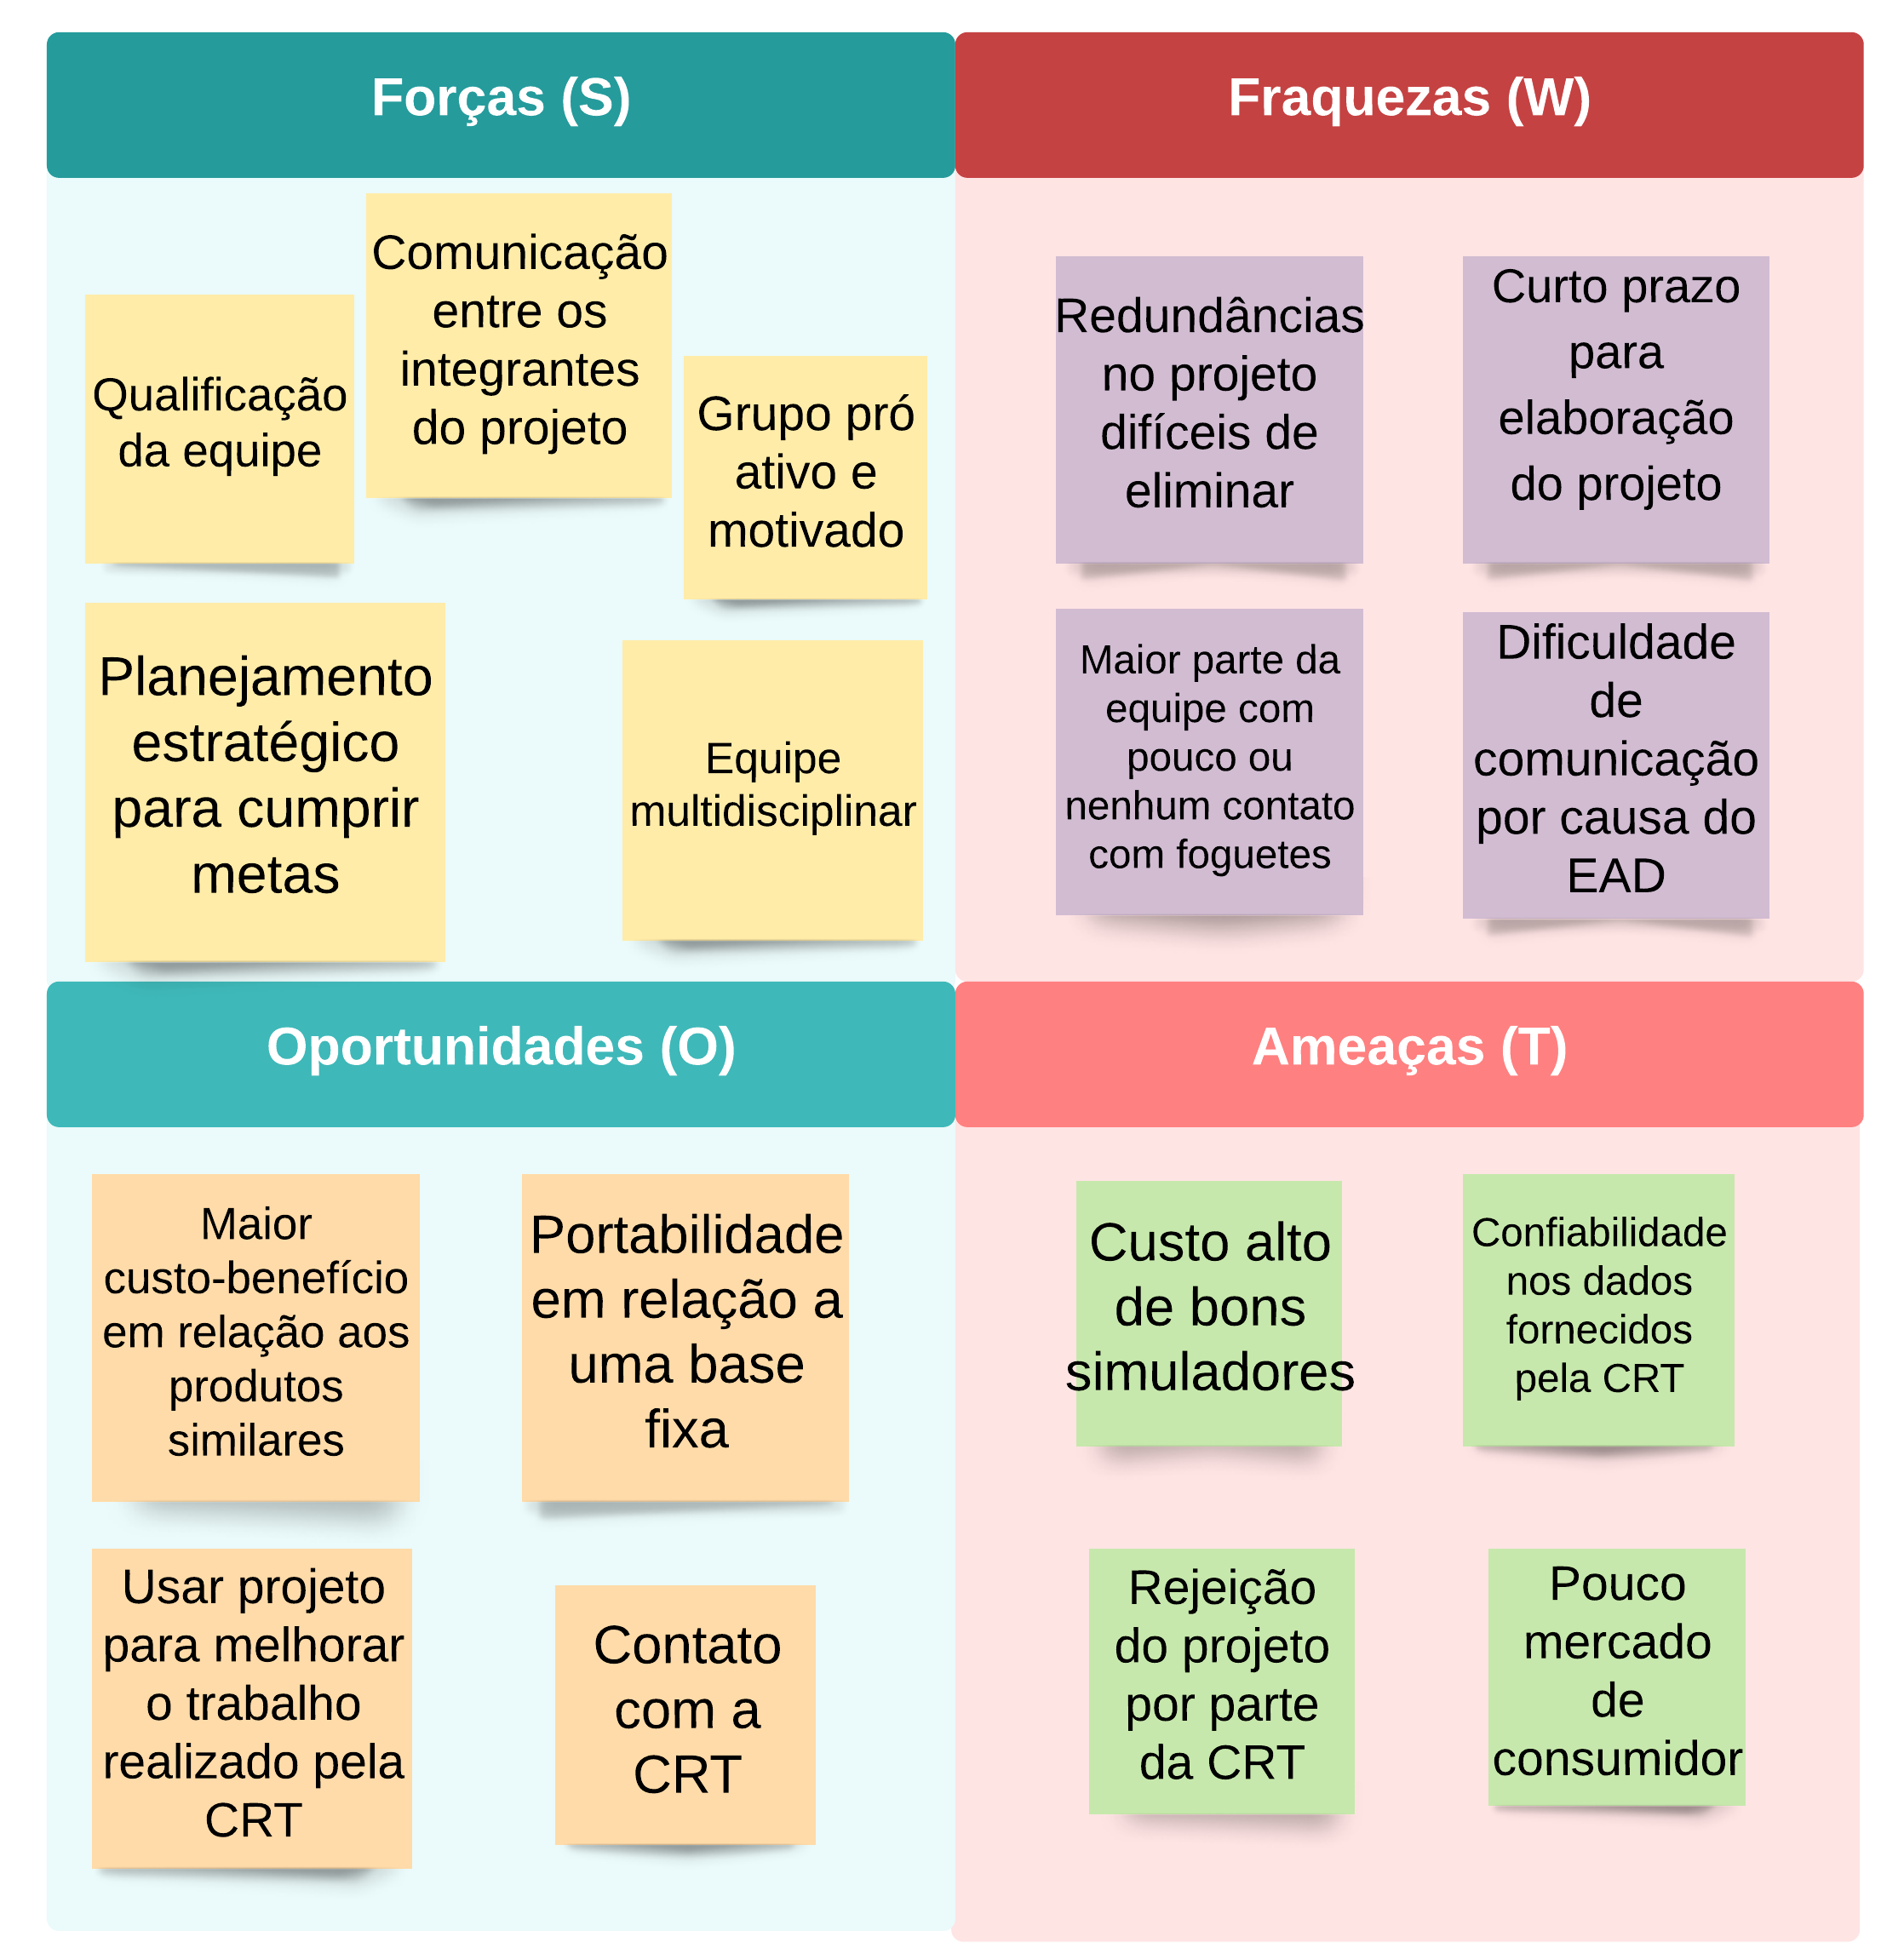
\includegraphics[scale=0.15]{figuras/SWOT_BaseLancamento.png}
  \caption{Matriz \textit{SWOT}. Matriz foi construída usando a ferramenta Lucidchart.} 
  \label{fig:matrizSWOT}
\end{figure}
\section{5W1H}

Antes de iniciar um projeto é muito importante ter com clareza: o que vai ser feito, como deve ser feito, porque deve ser feito, quem será responsável pelo trabalho, onde será feito e em qual período de tempo. A resposta para essas perguntas aprimoram o planejamento e auxiliam na criação de um plano de ação \cite{5w1hUFMG}.

A figura \ref{fig:5w1h} apresenta em forma de diagrama cada uma das 6 perguntas fundamentais e suas respectivas respostas baseadas no contexto desse projeto.

\begin{figure}[H]
  \centering
  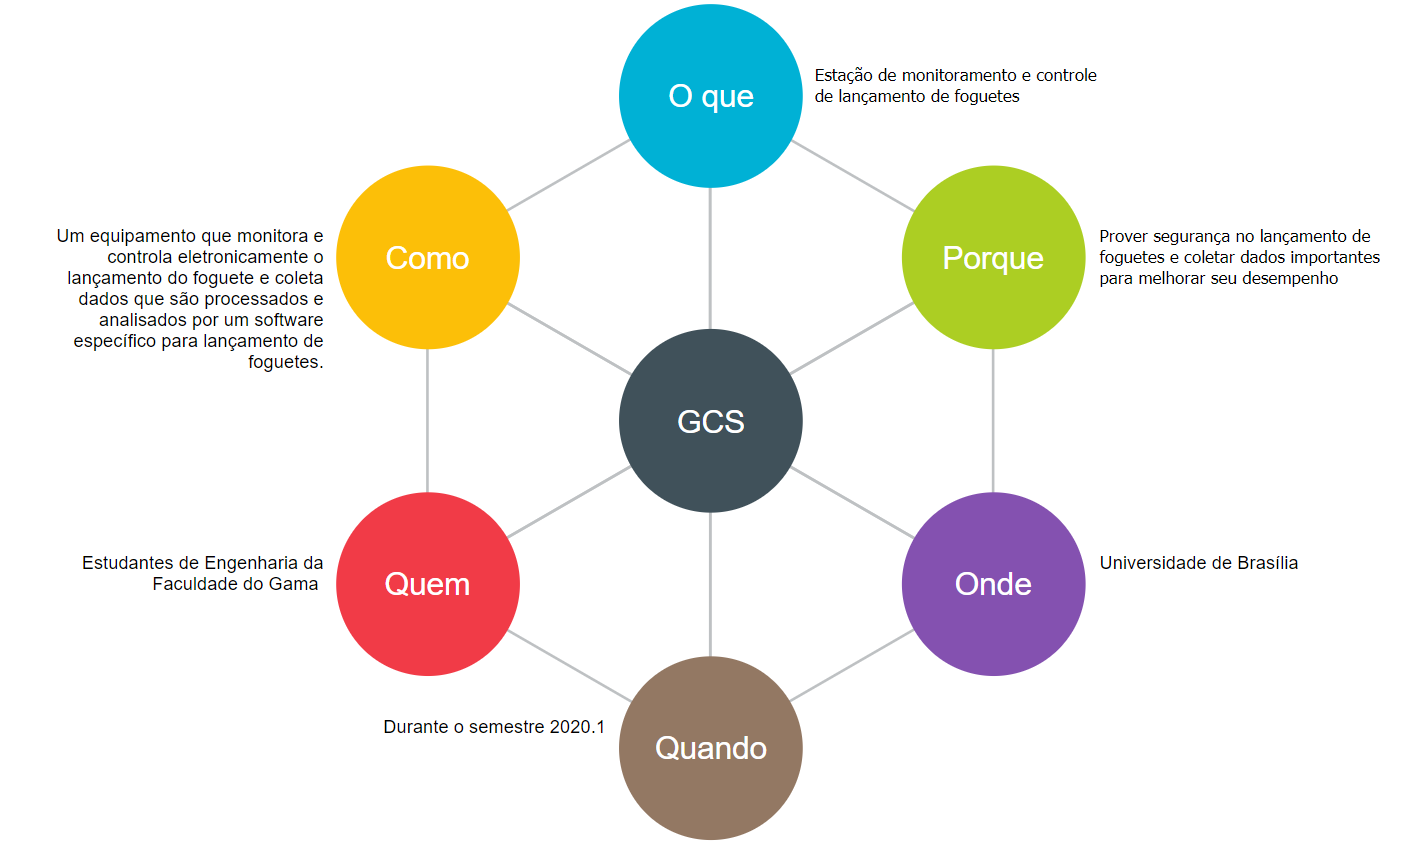
\includegraphics[width=\textwidth,height=\textheight,keepaspectratio]{figuras/5w1h.png}
  \caption{5W1H. O diagrama foi construído usando a ferramenta Visual Paradigm Online Diagrams.} 
  \label{fig:5w1h}
\end{figure}

\section{Bussines Model CANVAS}

Com o uso da ferramenta MIRO, foi desenvolvido um  \textit{business model} Canvas para o projeto, que pode ser visto no apêndice \ref{canvas}:  figura \ref{fig:Canvas} . Comumente chamado apenas de Canvas, essa ferramenta tem como objetivo esboçar a ideia de um modelo de negócio de maneira simples, eficaz e visual. Logo, um documento como este agrega valor ao projeto, devido ao fato deste estar ligado à uma equipe de competição.

Exemplificando, de acordo com o desempenho da equipe nas competições, a atenção dos outros competidores voltar-se-á ao projeto. Dada essa relação, poderão surgir  oportunidades de realizar negócios por meio do produto desenvolvido, assim justificando o desenvolvimento e o valor desse documento.  


\section{Estrutura Analítica do Projeto}

Com a necessidade de definir os objetivos e as entregas do projeto, foi criada a Estrutura Analítica do Projeto (EAP) na ferramenta \textit{Mindmeister}. O objetivo desse documento é fazer o planejamento de alto nível das atividades e dos objetivos do projeto, divididos em pacotes de entregas conhecidos como Pontos de Controle (PC). Esse documento será utilizado para fazer o planejamento das  \textit{sprints} de cada PC, para auxiliar na comunicação com os  \textit{Stakerholders}, pois ele detalha e define quais atividades e evoluções estão previstas para cada PC.

A EAP foi definida e acordada entre o Gerente Geral, o Diretor de Qualidade e os Diretores Técnicos. Levando em consideração as necessidades dos \textit{Stakerholders} e do contexto da disciplina. Como apresentado na Imagem \ref{fig:EAP}, o projeto está organizado em 3 pontos de controle, também conhecidos como \textit{Releases}, que consistem em pacotes de entrega que agreguem valor ao projeto e atendam às necessidades definidas no Plano de Ensino. Dentro de cada uma das entregas, estão as grandes frentes de desenvolvimento do Projeto, as quais são: Documentação/Viabilidade Técnica, Software, Eletrônica, Estrutura e Energia.

Em cada uma dessas frentes, estão definidas as atividades macro, ou os objetivos a serem alcançados e entregues nessa  \textit{Release}. Vale lembrar que a metodologia principal do projeto é Ágil, logo as atividades e objetivos podem ser alterados de acordo com a necessidade e a evolução do projeto.
\section{ \textit{Roadmap}}
Para uma melhor visualização e análise do  \textit{Roadmap}, ele pode ser visto no Apendice \ref{Roadmap}, mas também está disponível no link a seguir: \href{https://docs.google.com/spreadsheets/d/13mSpMqhIIh5OHl95djhCfA4ejr36CvJLpA65PvluUAU/edit?usp=sharing}{ \textit{Roadmap}}.

\subsection{Marcos Identificados}
\label{Milestones Identificados}
Os \textit{milestones} identificados encontram-se na tabela \ref{tab:tabelamilestones}. 




\begin{table}[H]
\begin{tabular}{|p{8cm}|p{6cm}|}
\hline
%%%%%%%%%%%%%%%%%%%%%%%%%%%%%%%%%%%%%%%%%%%%%%%%%
\textbf{Atividades}  & \textbf{Data de Entrega}         
\\ \hline
%%%%%%%%%%%%%%%%%%%%%%%%%%%%%%%%%%%%%%%%%%%%%%%%%

Entrega de Relatório Ponto de Controle 1    & 5 dias antes da apresentação
\\ \hline
%%%%%%%%%%%%%%%%%%%%%%%%%%%%%%%%%%%%%%%%%%%%%%%%%

Apresentação Ponto de Controle 1 &  18/09/2020, 25/09/2020 ou 02/10/2020

\\ \hline
%%%%%%%%%%%%%%%%%%%%%%%%%%%%%%%%%%%%%%%%%%%%%%%%%

Entrega de Relatório Ponto de Controle 2  & 5 dias antes da apresentação 
\\ \hline
%%%%%%%%%%%%%%%%%%%%%%%%%%%%%%%%%%%%%%%%%%%%%%%%%

Apresentação Ponto de Controle 2 & 16/10/2020, 23/10/2020 ou 30/10/2020
\\ \hline
%%%%%%%%%%%%%%%%%%%%%%%%%%%%%%%%%%%%%%%%%%%%%%%%%

Entrega de Relatório Ponto de Controle 3 & 5 dias antes da apresentação
\\ \hline
%%%%%%%%%%%%%%%%%%%%%%%%%%%%%%%%%%%%%%%%%%%%%%%%%
Apresentação Ponto de Controle 3 & 13/11/2020, 20/11/2020 ou 27/11/2020
\\ \hline
%%%%%%%%%%%%%%%%%%%%%%%%%%%%%%%%%%%%%%%%%%%%%%%%%
Entrega do repositório do projeto & 04/12/2020
\\ \hline
%%%%%%%%%%%%%%%%%%%%%%%%%%%%%%%%%%%%%%%%%%%%%%%%%
Apresentação de projetos na FIT/FGA On Line
(Feira de Inovação e Tecnologia da FGA) & 04/12/2020

\\ \hline
%%%%%%%%%%%%%%%%%%%%%%%%%%%%%%%%%%%%%%%%%%%%%%%%%
\end{tabular}
\caption{ \textit{Milestones} identificados.}
\label{tab:tabelamilestones}
\end{table}
\section{Viabilidade Técnica}
\label{recursosHumanos}
\subsection{Metodologia}

A fase inicial do projeto, também conhecida como Ponto de Controle 1 (PC1), visa garantir a definição da Metodologia, da gestão de riscos, e as definições que farão parte do desenvolvimento. Nesse projeto, 
o objetivo principal na definição da metodologia e da cultura é garantir o desenvolvimento e a organização da condução do projeto e das atividades de acordo com praticas da comunidade Ágil e do  \textit{DevOps} já adotadas pela comunidade \cite{licorish2016adoption}. 

As práticas do  \textit{DevOps} farão parte dos objetivos principais do PC1, pois irão auxiliar na gestão do projeto, baseando-se em quatro categorias: \textit{People, Process, Delivery e Runtime} \cite{leite2019survey}. Desde o primeiro momento, foram aplicados e apresentados conceitos e práticas do  \textit{DevOps},  \textit{Lean} e Ágil. Essas práticas irão auxiliar na adoção de uma nova cultura ágil e colaborativa entre os membros do projeto para garantir a qualidade nos produtos desenvolvidos. 

Além dos conceitos técnicos e não técnicos do  \textit{DevOps}, foi adotado como base o \textit{framework Scrum}, em que empregamos processos e técnicas aos papéis, eventos, artefatos e regras, adaptando as necessidades da equipe. O objetivo do \textit{Scrum} no projeto é permitir o controle do trabalho a ser realizado por meio de uma gestão dinâmica, assim identificar obstáculos durante o processo de desenvolvimento, e reagir a eles se torna mais fácil \cite{gren2015prospects} \cite{gren2020agile} \cite{licorish2016adoption}. A abordagem interativa e incremental empregada otimiza a previsão e monitoramento de riscos.

Também adotamos o uso do  \textit{Kanban} para controle do fluxo de produção da equipe. Para a otimização do trabalho desta, foi utilizada a ferramenta  \textit{Trello}, já integrada no  \textit{MsTeams}. 

Para rastrear as tarefas e levantar dados, utilizamos o  \textit{Dashio} para coleta de Métricas e Indicadores que auxiliem as equipes. As Imagens \ref{fig:cumulativesoftware}, \ref{fig:cumulativeeletronica} e \ref{fig:cumulativeestrutura} apresentam o Gráfico \textit{Cumulative Flow} desse PC1 (Sprint 0 até 3). Pelo gráfico, podemos observar as entregas feitas a cada \textit{Sprint} (avanço no gráfico a cada 7 dias). O objetivo do time é reduzir o tempo entre as entregas para que não seja em formato de "pacotes" ao fim de cada revisão, garantindo assim uma entrega contínua. É possível observar que todos os times conseguiram fazer entregas durante a  \textit{sprint} e que na Imagem \ref{fig:cumulativesoftware} e \ref{fig:cumulativeeletronica} existem algumas distorções nos gráficos, pois os times identificaram duplicidade de atividades e arquivaram os \textit{Cards}.

\begin{figure}[H]
    \centering
  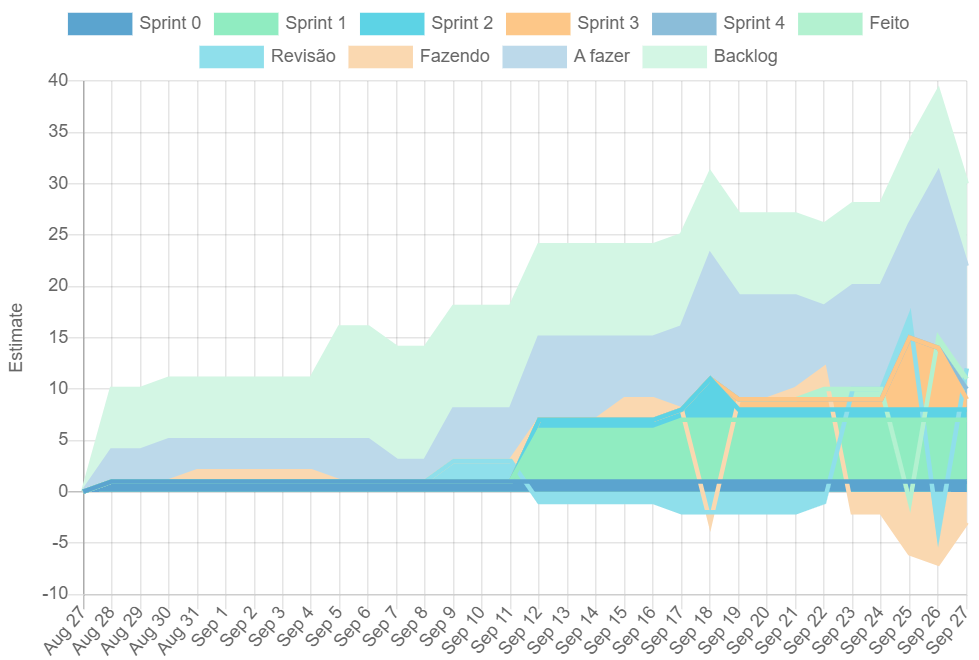
\includegraphics[scale=0.3]{figuras/cumulative_software.png}
  \caption{\textit{Cumulative Flow} da equipe de Software coletados de 27 de agosto até 26 de setembro de 2020.}
  \label{fig:cumulativesoftware}
\end{figure}
\begin{figure}[ht]
\centering
  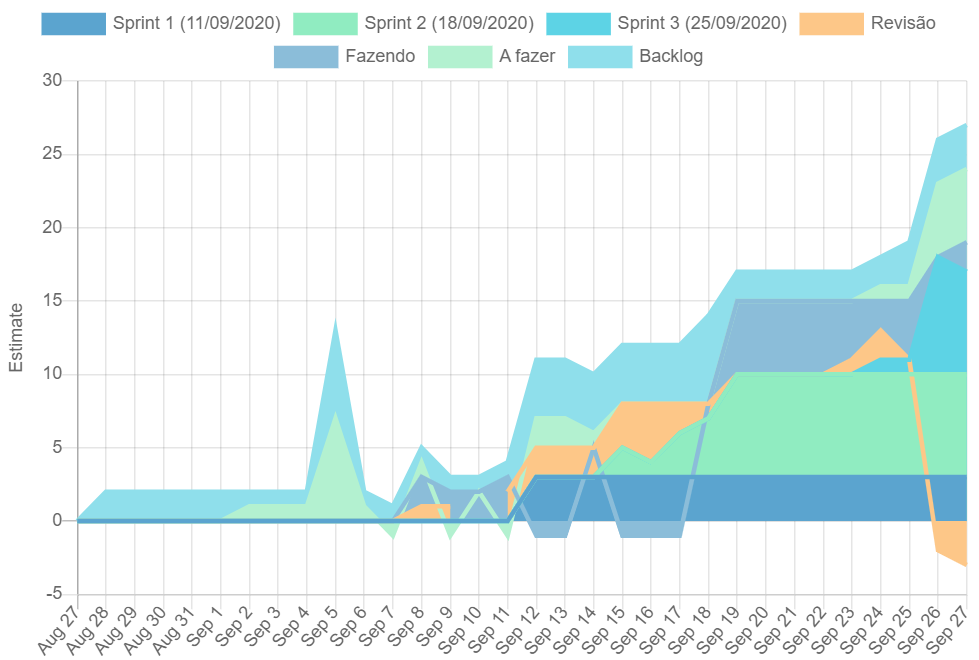
\includegraphics[scale=0.3]{figuras/cumulative_eletronica.png}
  \caption{\textit{Cumulative Flow} da equipe de Eletrônica coletados de 27 de agosto até 26 de setembro de 2020.}
  \label{fig:cumulativeeletronica}
\end{figure}
\begin{figure}[H]
\centering
  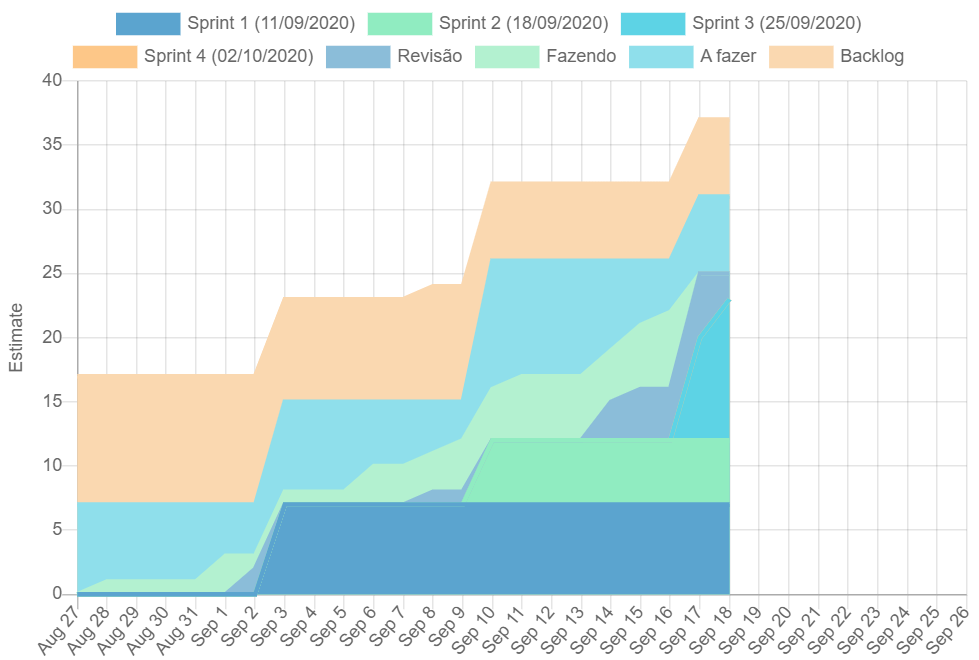
\includegraphics[scale=0.3]{figuras/cumulative_estrutura.png}
  \caption{\textit{Cumulative Flow} da equipe de Estrutura e Energia coletados de 27 de agosto até 26 de setembro de 2020.}
  \label{fig:cumulativeestrutura}
\end{figure}

Já o XP foi uma das metodologias adotadas pelo conjunto de práticas que são ditas como boas na Engenharia de Software como pareamento, refatorar o tempo todo, testar o tempo todo, entre outros.

\subsection{Papeis}
Durante o projeto, a equipe possuirá um Gerente Geral, um Diretor de Qualidade e será subdividida em 3 subgrupos, cada um contando com um Diretor Técnico (destacado em negrito):
\begin{itemize}
    \item Gerente Geral: Isaque Alves de Lima
    \item Diretor de Qualidade: Diogo Filipe Sens
    \item Estrutura e Energia
        \subitem - \textbf{Luisa Prospero de Carvalho Silva}
        \subitem - Artur Cardoso de Almeida
        \subitem - Douglas Alves Brandão 
        \subitem - Milena Martins Magalhães
        \subitem - Thainá Rodrigues Fernandes
    \item Eletrônica
        \subitem - \textbf{Gustavo Cavalcante Linhares}
        \subitem - Francisco Matheus Fernandes Gomes 
        \subitem - Misael de Souza Andrade
    \item Software
        \subitem - \textbf{João Henrique Egewarth}  
        \subitem - Andre Hernandez Bargas
        \subitem - Augusto Moreno Vilarins
        \subitem - Gabriela Alves da Gama
\end{itemize}

\subsection{Ritos Adotados}
\label{ritos}
\begin{itemize}
    \item \textit{Sprint}
        \subitem Início: sexta-feira
        \subitem Fim: sexta-feira
        \subitem Duração: 7 dias
\end{itemize}

\subsubsection{Planejamento da \textit{Sprint}}

\textbf{Duração máxima: 45 min}

A reunião de planejamento da  \textit{Sprint} é realizada semanalmente às sextas-feiras com a participação de todos os participantes separados nas suas frentes. A reunião de planejamento segue os seguintes passos:


1 - O time discute quais são as prioridades e necessidades do time;

2 - O time deve ter um objetivo bem definido para a  \textit{sprint};

3 - O time cria e seleciona as atividades que devem ser produzidas durante a  \textit{sprint};

\textbf{OBS:} Como as  \textit{sprints} são semanais, as atividades devem ser pensadas para concluir em 7 dias.

4 - Caso haja, o time deve definir e apresentar o pareamento da semana;

\textbf{OBS:} Esse pareamento deverá estar no definido na  \textit{issue}.

5 - Criar os  \textit{cards} no  \textit{Trello};

Deve conter nas  \textit{issues}:

- Titulo;

- Breve descrição;

- Responsável (no mínimo um);


\begin{itemize}
    \item\textbf{Entradas}
        \subitem \textit{Backlog} do produto;
        \subitem Último Incremento do produto;
        \subitem Desempenho na última \textit{Sprint}.
    
    \item\textbf{Saída}
        \subitem \textit{Backlog} da \textit{Sprint}.
\end{itemize}   


\subsubsection{Revisão da \textit{Sprint}}
\textbf{Duração máxima: 45 min}

\textbf{Missão:} Inspecionar o incremento e adaptar o \textit{Backlog}.

A reunião de Revisão do time é realizada semanalmente às sextas-feiras com a participação de todos os membros do time. A reunião segue os seguintes passos:

1 - O time discute e valida as atividades e artefatos produzidos durante a  \textit{sprint} que se finaliza;

2 - O time discute o \textit{Backlog} do Produto atual e se o time conseguirá atingir a meta das entregas;

3 - O grupo colabora com as soluções;

4 - É feita uma análise do mercado para definir o que é mais importante para fazer a seguir.


\subsubsection{Retrospectiva da \textit{Sprint}}
\textbf{Duração máxima: 30 min}


1 - Revisar, dentro do modelo de trabalho e das práticas do processo do  \textit{Scrum}, o processo de desenvolvimento, de forma a torná-lo mais eficaz e gratificante para a próxima \textit{Sprint};

2 - Inspecionar como correu a última \textit{Sprint} em se tratando de pessoas, das relações entre elas, dos processos e das ferramentas;

3 - Priorizar os principais itens que correram bem e aqueles que, se feitos de modo diferente, poderiam ter deixado as coisas ainda melhores.


\subsection{Ferramentas}
\begin{itemize}
    \item Teams
        \subitem Principal ferramenta de comunicação que permite o compartilhamento de vídeos, documentos e a integração com as outras ferramentas utilizadas no projeto, além de centralizar a comunicação ela é a ferramenta principal para as conferências.
    \item Drive
        \subsubitem Ferramenta em nuvem para armazenamento compartilhado. Será utilizada para compartilhar a documentação e informações entre os membros.
    \item Overleaf
        \subsubitem É uma ferramenta colaborativa de escrita online em LaTeX, cujo objetivo é facilitar todo o processo de escrita, edição e publicação de documentos.
    \item GitHub
        \subsubitem O GitHub é uma plataforma de hospedagem de código-fonte com controle de versão usando o Git.
\end{itemize} 
\section{Gestão dos Riscos}
\label{levantamentoRiscos}

A Gestão de Risco é um processo de identificação, análise, avaliação, tratamento e monitoramento de um evento que pode atrasar uma entrega de um produto ou serviço. A ISO 31000 define como atividades coordenadas para dirigir e controlar uma organização no que se refere a riscos \cite{purdy2010iso}.
Neste projeto, a gestão de risco é feita utilizando práticas da metodologia ágil, onde os riscos Técnicos, Externos, Organizacionais e relacionados ao Gerenciamento são levantados e acompanhados a cada  \textit{Sprint}, a fim de reduzir a probabilidade do risco acontecer \cite{cohn_RiskBurndown_blog2010}.

Para isso, criamos um \textit{burndown} de Riscos que auxilia no acompanhamento dos riscos por \textit{Sprints}, verificando a probabilidade e o impacto do risco, a fim de reagir a tempo. Esse modelo de gestão de riscos baseia-se em uma métrica subjetiva, pois o próprio time define o impacto e a probabilidade do risco acontecer. 

O processo de identificação, análise, avaliação, tratamento e monitoramento de um evento (interno ou externo) que pode ser um risco para o projeto é feito em todas as {\em sprints}, sendo que cada {\em sprint} cobre o período de uma semana. Primeiramente, é feito um levantamento de todos os $N$ eventos potenciais de risco ao projeto. Cada item desse levantamento é avaliado periodicamente, levando-se em conta dois fatores: a chance de o risco ocorrer $P$ e o impacto disso $I$. No nosso caso, ambos fatores ($P$ e $I$) são anotados usando valores que vão de 0 a 5, indicando as seguintes avaliações qualitativas de probabilidade de cada evento ocorrer: nenhum; raro; improvável; pouco provável; 
muito provável; quase certo. Os cálculos e o acompanhamento dos riscos estão disponíveis na planilha de Riscos por meio do link a seguir: \href{https://docs.google.com/spreadsheets/d/1TQ4I9uqX-XxH3AdRi01n4jIX4YpIWYOHws1GxpdqUF0/edit?usp=sharing}{Planilha de Acompanhamento dos Riscos}.

\begin{figure}[ht]
  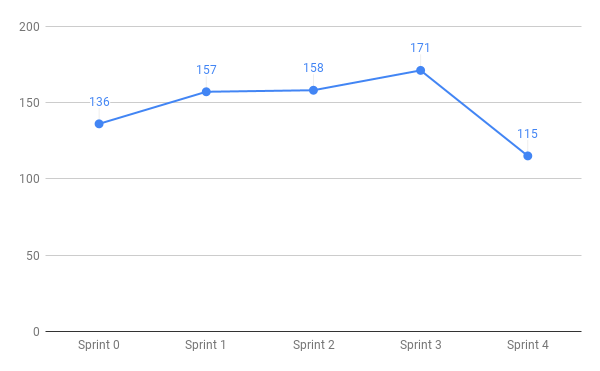
\includegraphics[scale=0.75]{figuras/burndownrisco.png}
  \caption{\textit{Risk Burndown} geral: multiplição da  probabilidade do evento do risco pelo impacto do evento no desenvolvimento do projeto, durante a Release 1.} 
  \label{fig:riscogeral}
\end{figure}

O fator {\em Risk Burndown} (eixo Y no gráfico da figura \ref{fig:riscogeral}) é calculado multiplicando-se esses dois fatores e somando os resultados para todos os $N$ eventos avaliados.
Até o momento, foram identificados $N=17$ fatores de risco, ou seja, o maior valor possível para o fator {\em risk burndown} deste projeto atualmente seria de $N \times P \times I = 17 \times 5 \times 5 = 425$, num cenário de caos absoluto.
Porém, não é de se esperar que todos os fatores tenham impacto máximo e máxima probabilidade de acontecer ao mesmo tempo, por isso o gráfico da figura \ref{fig:riscogeral} mostra o eixo Y indo somente até 200.

Durante a análise da probabilidade, são definidas ações para mitigar o risco. Desde o início do projeto, os principais riscos foram ligados à cultura e organização das atividades, definição do escopo para atender às necessidades do cliente e à pandemia. É possível notar o crescimento de risco do projeto na {\em Sprint} 3, devido a identificação de novos riscos, mas é possível notar na Imagem \ref{fig:riscogeral} que os riscos estão diminuindo constantemente.
\section{Estimativa de Custos}

Apesar de não existir a necessidade de construção do projeto este semestre, devido a situação sanitária no qual o mundo se encontra, foi construído uma tabela com os custos totais dos materiais componentes que seriam utilizados. A tabela \ref{tab:estimativa materiais} mostra um valor estimado do metro quadrado dos materiais pesquisados. 

\begin{table}[H]
\begin{tabular}{| m{4cm}|m{2cm}|m{2cm}|m{2cm}|m{2cm}|m{2cm}|}
\hline
\multicolumn{6}{|c|}{\textbf{Estrutura e Energia}}\\
\hline
Material & Preço  & Quantidade & Frete & Loja & Total  \\ 
\hline
Bateria Lítio Ferro Fosfato (UPLFP12-30) & 1.426,00  & 1 & 00,00 & Unipower & 1.426,00  \\ 
\hline
Módulo Regulador de Tensão (LM2596)   & 10,90  & 3  & 21,11 & Curto Circuito      & 53,81  \\ 
\hline
MDF   &  R\$36,81 & 1$m^2$x3mm  &   &    &  R\$36,81 \\ 
\hline
MDF   & R\$62,50  & 1$m^2$x6mm  &   &    & R\$62,50  \\ 
\hline
PRFV   & R\$52,90  & 1$m^2$  &   &    &  R\$52,90 \\ 
\hline
PRFC   &  R\$421,43 & 1$m^2$ &   &    &  R\$421,43 \\ 
\hline
PLA   & R\$140,00  & 1kg  &   &    &  R\$140,00  \\ 
\hline
ABS   &  R\$ 16,80 & 1kg  &   &    & R\$ 16,80  \\ 
\hline
 Atuador pneumático  &  entre R\$250 a R\$2000 & 2  &   &    &   \\ 
\hline
 Atuadores elétricos  & entre U\$60 a U\$240  &  2 &   &    &   \\ 
\hline

\end{tabular}
\caption{Estimativa de custos de Materiais}
\label{tab:estimativa materiais}
\end{table}

\begin{table}[H]
\begin{tabular}{| m{6cm}|m{1cm}|m{2cm}|m{1cm}|m{3cm}|m{1cm}|}
\hline
\multicolumn{6}{|c|}{\textbf{Eletrônica}}                                                 \\ \hline
Componente                & Preço  & Quantidade & Frete & Loja          & Total  \\ \hline
Jetson Nano Developer Kit  & 899,91 & 1          & 50,45 & Submarino    & 950,36 \\ \hline
TELA LCD - 9 polegadas    & 269,75 & 1          & 0,00  & arduoeletro   & 269,75 \\ \hline
Mini Teclado com touchpad & 189,14 & 1          & 0,00  & Mercado Livre & 189,14 \\ \hline
Placa LoRa Esp32          & 129,90 & 3          & 27,90 & Mercado Livre & 417,60 \\ \hline
Sensor BMP280             & 13,50  & 1          & 21,11 & Curtocircuito & 34,61  \\ \hline
Célula de carga 50kg      & 16,90  & 1          & 16,50 & Eletrogate    & 33,40  \\ \hline
Módulo Hx711              & 10,40  & 1          & 19,90 & Mercado Livre & 30,30  \\ \hline
Módulo GPS GY-NEO6MV2     & 79,90  & 1          & 19,70 & Robocore      & 99,60  \\ \hline
\end{tabular}
\caption{Estimativa de custos componentes eletrônicos}
\end{table}



Com isso o custo total dos materiais do projeto inicialmente é\textbf{ R\$ 3.504,57} reais.


